\documentclass[a4paper]{article} 
\addtolength{\hoffset}{-2.25cm}
\addtolength{\textwidth}{4.5cm}
\addtolength{\voffset}{-3.25cm}
\addtolength{\textheight}{5cm}
\setlength{\parskip}{0pt}
\setlength{\parindent}{0in}

\usepackage{natbib}
\usepackage{blindtext} % Package to generate dummy text
\usepackage{charter} % Use the Charter font
\usepackage[utf8]{inputenc} % Use UTF-8 encoding
\usepackage{microtype} % Slightly tweak font spacing for aesthetics
\usepackage{amsthm, amsmath, amssymb} % Mathematical typesetting
\usepackage{float} % Improved interface for floating objects
\usepackage{hyperref} % For hyperlinks in the PDF
\usepackage{graphicx, multicol} % Enhanced support for graphics
\usepackage{xcolor} % Driver-independent color extensions
\usepackage{pseudocode} % Environment for specifying algorithms in a natural way
\usepackage[ddmmyyyy]{datetime} % Uses YEAR-MONTH-DAY format for dates
%\usepackage{gensymb}
\usepackage{bibentry}

\usepackage{fancyhdr} % Headers and footers
\pagestyle{fancy} % All pages have headers and footers
\fancyhead{}\renewcommand{\headrulewidth}{0pt} % Blank out the default header
\fancyfoot[L]{} % Custom footer text
\fancyfoot[C]{} % Custom footer text
\fancyfoot[R]{\thepage} % Custom footer text
\newcommand{\note}[1]{\marginpar{\scriptsize \textcolor{red}{#1}}} % Enables comments in red on margin

%----------------------------------------------------------------------------------------

\usepackage{adjustbox}
\usepackage{float}
\usepackage{multicol}
%-------------------------------
%	TITLE VARIABLES (identify your work!)
%-------------------------------

\newcommand{\yourname}{Jakob Kralj 4.A} % replace YOURNAME with your name
\newcommand{\papertitle}{Ravnovesje navorov} % replace X with paper title

\begin{document}

%-------------------------------
%	TITLE SECTION (do not modify unless you really need to)
%-------------------------------
\fancyhead[C]{}
\hrule \medskip
\begin{minipage}{0.295\textwidth} 
\raggedright
\footnotesize
\yourname \hfill\\ 
\end{minipage}
\begin{minipage}{0.69\textwidth} 
\centering 
\Large
\text{\papertitle}\\ 
\normalsize 
\end{minipage}
\medskip\hrule 
\bigskip


%-------------------------------
%	ASSIGNMENT CONTENT (add your responses)
%-------------------------------

\section*{Naloga:} % this is an example

Preveri ali je v ravnovesju vsota vseh navorov nič.

\section*{Potrebščine:}

Stojalo, prečka, uteži z vrvicami, meter.

\section*{Skica:}

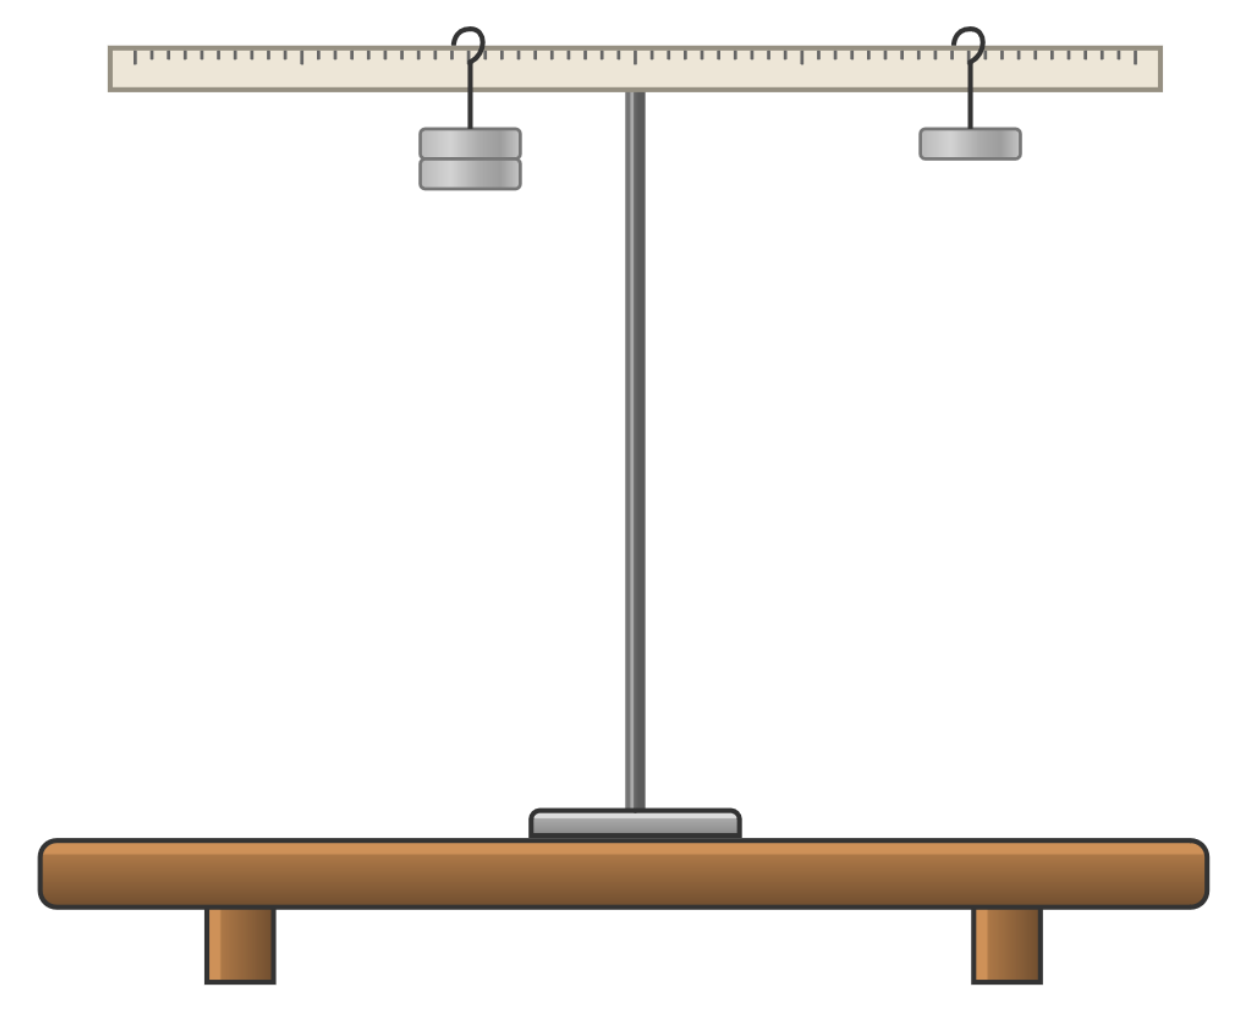
\includegraphics[scale=0.5]{skica.png}

\section*{Meritve:}

Sestavi stojalo in nanj vrtljivo vpni prečko. Na levo in desno stran osi obesi uteži z različnimi masami tako, da bo prečka v ravnovesju. Izmeri razdalje prijemališč tež uteži od osi in jih vpiši v tabelo. Prav tako zapisuj v tabelo tudi teže uteži. Opravi pet meritev. Za vsako meritev izračunaj navor na levi ter navor na desni strani osi. Zapiši ju v tabelo.


\begin{table}[H]
\centering
\renewcommand{\arraystretch}{1.5}
\begin{tabular}{lllll}
   & $m_1 [g]$ & $r_1 [cm]$ & $m_2 [g]$ & $r_2 [cm]$ \\
1 & 50,0  & 12,0 & 25,0 & 23,5 \\
2 & 100,0 & 9,0  & 50,0 & 18,0 \\
3 & 100,0 & 5,9  & 25,0 & 23,0 \\
4 & 150,0 & 7,0  & 50,0 & 21,0 \\
5 & 125,0 & 3,7  & 25,0 & 18,5
\end{tabular}
\end{table}



\section*{Rezultati in obdelava podatkov:}


   $M$ lahko izračunamo s pomočjo enačbe (v primeru da sta vektorja razdalje in težnega pospeška pravokotna):
   \begin{equation}
      M = m*g*r
   \end{equation}

   
   Kjer lahko uporabimo parametre:
   \begin{gather}
      g = 9.81 [\frac{m}{s^2}]
   \end{gather}

Rezultati:
\begin{table}[H]
   \centering
   \renewcommand{\arraystretch}{1.5}
   \begin{tabular}{lllllll}
      & $m_1 [g]$ & $r_1 [cm]$ & $m_2 [g]$ & $r_2 [cm]$ & $M_1 [Nm]$ & $M_2 [Nm]$ \\
   1 & 50,0  & 12,0 & 25,0 & 23,5 & 0,059 & 0,058 \\
   2 & 100,0 & 9,0  & 50,0 & 18,0 & 0,088 & 0,088 \\
   3 & 100,0 & 5,9  & 25,0 & 23,0 & 0,058 & 0,056 \\
   4 & 150,0 & 7,0  & 50,0 & 21,0 & 0,103 & 0,103 \\
   5 & 125,0 & 3,7  & 25,0 & 18,5 & 0,045 & 0,045
\end{tabular}
\end{table}

Rezultati se skaldajo z največjo napako $4\%$
\section*{Interpretacija:}

Napake so skoraj zanemarljive, večinoma posledica nenatančnosti v tehtanju in merjenju. Zaradi trenja obstaja možnost da prečka ni bila popolnoma v ravnotežju. 

\section*{Dodatek}
Uporabi ugotovitve o vsoti navorov v ravnovesju v naslednjem primeru.
\subsection*{Potrebščine}
2 tehtnici, prečka z merilom, uteži.
\subsection*{Skica}
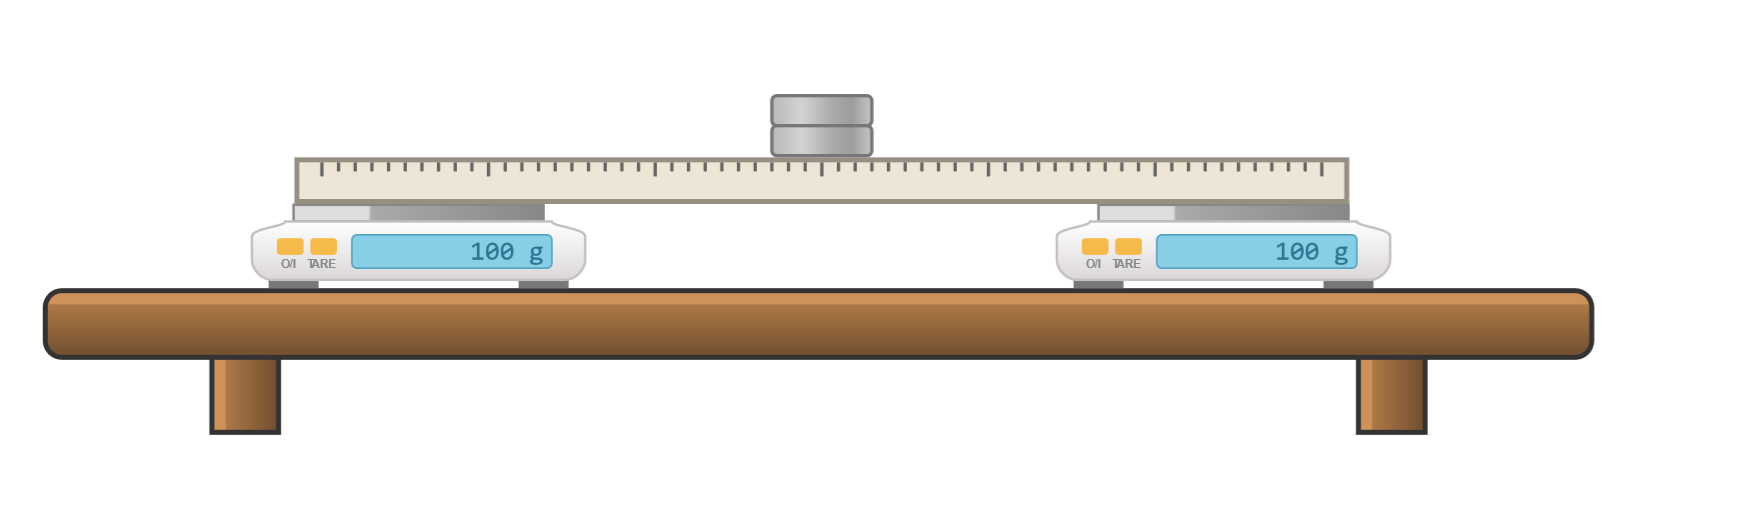
\includegraphics[scale=0.5]{dodatek_skica.png}
\subsection*{Meritve}
Vajo sestavi po sliki. Nato na prečko položi utež (lahko več) z znano maso. Odčitaj lego uteži ter sili podpor, ki ju določiš s tehtnicama. Meritev opravi za tri različne lege različnih uteži.
\begin{equation}
   m = 200g
\end{equation}
\begin{center}
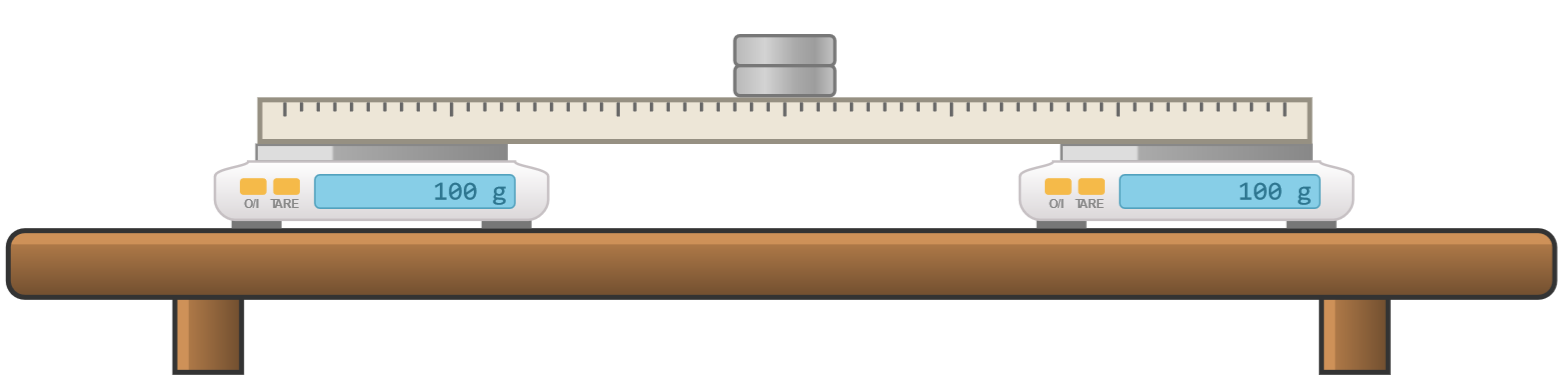
\includegraphics[scale=0.4]{primer1.png}
\begin{gather}
   \frac{m g r}{2} = F_1 r \\
   F_1 = \frac{mg}{2} \\
   F_1 = 0.98N
\end{gather}
\end{center}
\begin{center}
   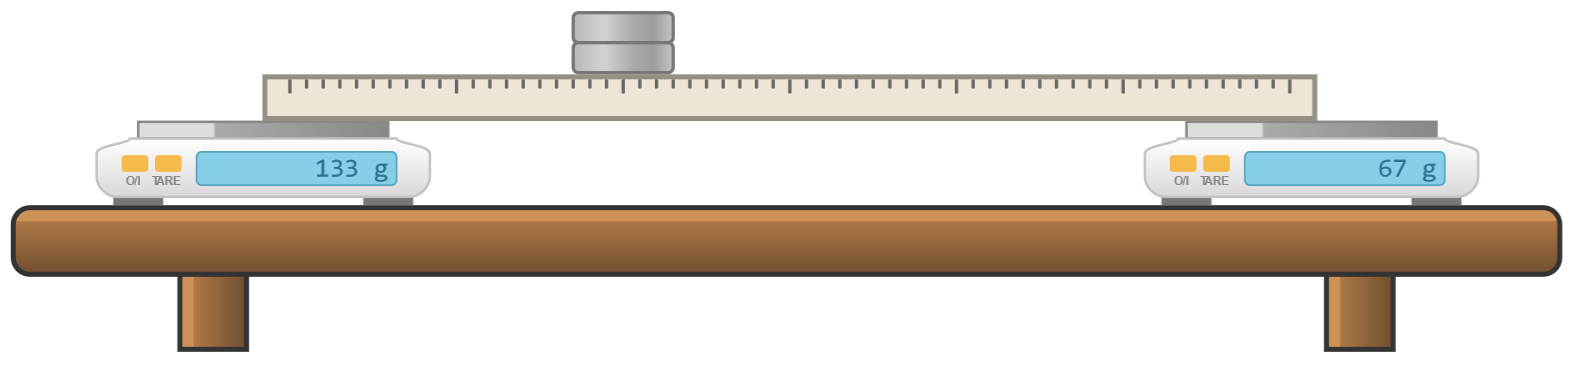
\includegraphics[scale=0.4]{primer2.png}
   \begin{gather}
      \frac{m g r}{3} = F_2 r \\
      F_2 = \frac{mg}{3} \\
      F_2 = 0.65N
   \end{gather}
\end{center}
\begin{center}
   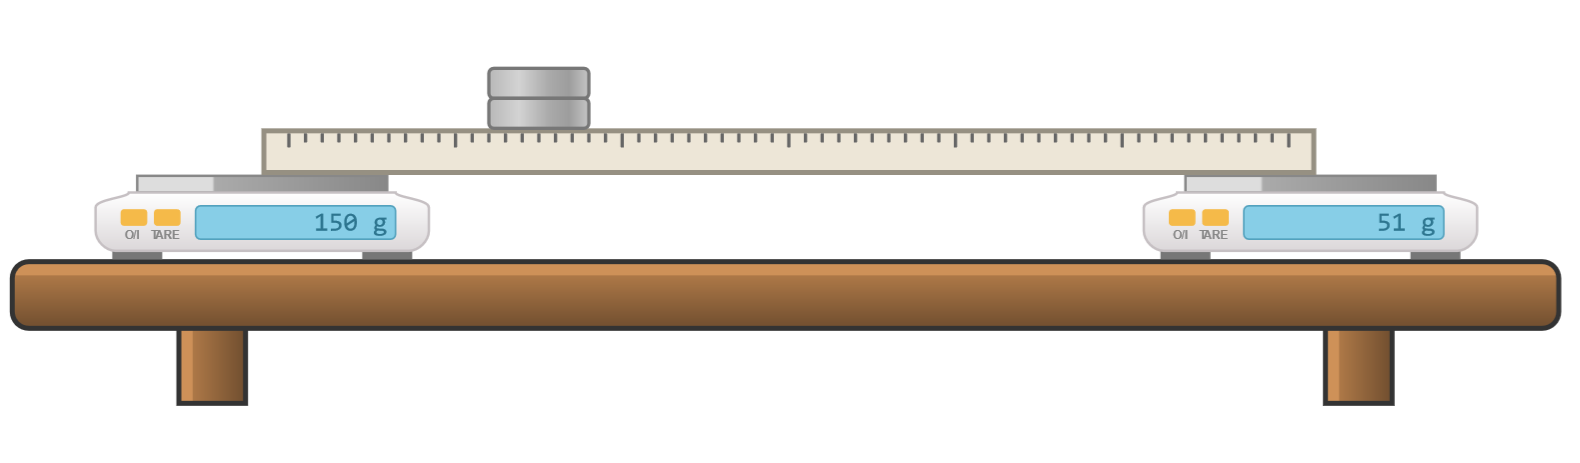
\includegraphics[scale=0.4]{primer3.png}
   \begin{gather}
      \frac{m g r}{4} = F_3 r \\
      F_3 = \frac{mg}{4} \\
      F_3 = 0.49N
   \end{gather}
\end{center}
\subsection*{Interpretacija}
Izračunane sile se ujemajo z izmerjenimi, vendar pa so navadno manjše zaradi neupoštevanja teže palice. Napake so posledica tudi včasih nepreveč natančne postavitve palice, kjer lahko pozicija palica ne na sredini vpliva na $r$.
\end{document}